\subsection{Einleitung}
Der signifikanteste Unterschied zwischen üblichen Dateisynchronisationsdiensten
und \sblit besteht im Verzicht eines Servers. Anders als im Kapitel 1.1.2. erklärt,
findet die Datenübertragung bei \sblit zwischen zwei Endgeräten nicht über einen Server statt,
sondern über eine direkte verschlüsselte Verbindung zwischen diesen zwei Geräten.

Durch diesen Ansatz fällt die zentrale Sammelstelle von Nutzerdaten
weg und dem Datendiebstahl von Hackern wird ein Riegel vorgeschoben. Außerdem
wird kein betreibendes Unternehmen mehr benötigt, um Server zu warten, womit auch
die einheitliche Anlaufstelle für staatliche Sicherheitsbehörden und Geheimdienste
nicht mehr existiert.

\subsection{Herausforderungen}
\subsubsection{Allgemein}
Mit dem Weglassen eines Servers, entstehen aber auch viele Herausforderungen,
wenn der volle Funktionsumfang eines üblichen Dateisynchronisationsdienstes
trotzdem gewährleistet werden soll.

\subsubsection{Verbindungsaufbau zwischen Clients}
So fehlt der öffentliche Server als bekannter \glqq{} Mittelmann \grqq{} in der Kommunikation
zwischen den Clients, sodass sich diese über das Internet hinwegüber mit einem
eigenen Protokoll finden, um eine direkte Verbindung erfolgreich aufbauen zu können.
Mehr zu den genauen Herausforderungen beim Verbindungsaufbau und
die Bewältigung dieser folgt im Kapitel \ref{ch:Partnerschaften}.

\subsubsection{Alternative zu Server als \gls{filecloud}}
Der Server agiert aber nicht aber nicht nur als \glqq{} Mittelmann \grqq{} damit die
Clients miteinander kommunizieren können. Er dient nämlich auch als \gls{filecloud},
also als Zwischenspeicher für Daten. Dieser ist nämlich essenziell, wenn man
Dateien ohne große Komplikationen synchronisieren will. Um zu erklären warum das
so ist, gehen wir von folgendem Szenario bei Verwendung eines Servers aus:
Der Rechner in der Schule ist eingeschaltet, das Gerät zu Hause nicht. Wird nun
eine bereits synchronisierte Datei auf dem Schulrechner bearbeitet, wird eine Kopie dieser wie
üblich auf die \gls{filecloud}, also den Server hochgeladen. Wenn die Schule vorbei ist,
wird der Schulrechner abgedreht und zu Hause kann sofort die neuste Version der
geänderten  Datei beim Einschalten des Heim-PCs übertragen werden, obwohl der
Schulrechner ausgeschaltet ist, da die Datei in der \gls{filecloud}
zwischengespeichert wurde und sie von dort aus gesendet wurde.
\begin{figure}[h]
	\centering
  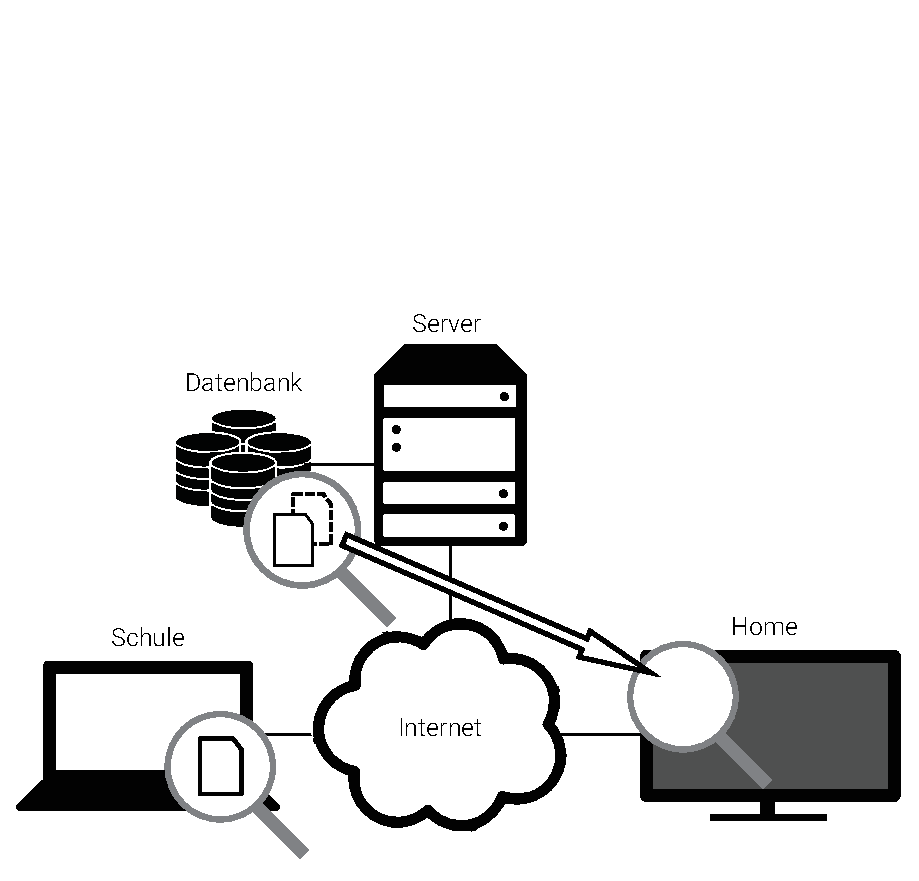
\includegraphics[]{images/dropbox_temp_1}
  \caption{Heimrechner ist nicht erreichbar. Die Datei kann nicht mit ihm
	synchronisert werden}.
\end{figure}
\begin{figure}[h]
	\centering
  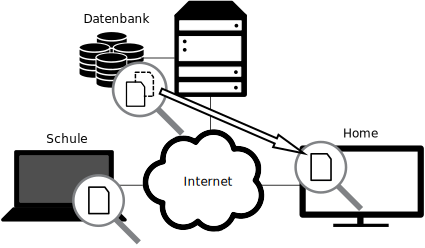
\includegraphics[]{images/dropbox_temp_2}
  \caption{Heimrechner ist wieder erreichbar, sodass die Datei nun vom Server
	bezogen werden kann}.
\end{figure}

Ohne den Server als \gls{filecloud}, wäre die alte Version der Datei bearbeitet worden, sodass zwei
neue Versionen der Datei existieren würden. Dies nennt man einen \gls{versionconflict}.
%TODO Bild einfügen, auf dem bei sblit ein Client nicht erreichbar ist.
Mit dem Verzicht auf den Server, muss also eine alternative \gls{filecloud} benutzt
werden, um Dateien zwischenspeichern zu können, sodass in vorherigen Szenario ohne Server
keine \glspl{versionconflict} auftreten.

Deshalb kommt bei \sblit eine dezentrale \gls{filecloud} zum Einsatz. Anstelle
eines zentralen Speicherns durch einen Server, wird auf den Speicherplatz der
verschiedenen Nutzern von \sblit zurückgegriffen. Diese dezentrale \gls{filecloud}
besteht also aus den verteilten Speicherplätzen verschiedenster Nutzer.

Dieses Prinzip funktioniert durch ein \gls{p2pnet}, welches durch faire Abkommen zwischen den \sblit-Nutzern realisiert wird,
sogenannten \glspl{partnership}. Grundsätzlich sind \glspl{partnership} einfach eine
Vereinbarung mit anderen, teilweise sogar fremden Nutzern, sich gegenseitig Speicherplatz
freizugeben. Eine \gls{partnership} wird entweder automatisch mit unbekannten Nutzern
geschlossen, oder durch den Nutzer selbst mit Bekannten. Genauer wird auf dieses Thema allerdings weiter hinten im Buch im
Kapitel \ref{sec:Partnerschaften} eingegangen.

Die Dateien werden aber natülich nicht nach einer verschlüsselten Übertragung unverschlüsselt
auf den teilweise fremden \glspl{partnerdevice} gespeichert. Verschlüsseln ist dabei
natürlich Pflicht, es wurde allerdings noch einen Schritt weiter gedacht. Generell
hat bei \sblit nämlich nur der Nutzer, dem der die Datei auf den Partnergeräten speichert und
dessen \glspl{syncpartner} Zugriff auf die vollständigen Dateien.

Wenn also mindestens ein \gls{syncpartner} nicht erreichbar ist und die Datei somit
nicht direkt über eine verschlüsselte Verbindung übertragen werden kann, wird eine Kopie
dieser Datei in viele Datenblöcke aufgeteilt. Diese Blöcke werden verschlüsselt und
verstreut auf den \glspl{partnerdevice} gespeichert.

Für die Nutzer hinter den \glspl{partnerdevice} ist es somit unmöglich auf die ursprüngliche
Datei zu schließen. Einerseits, ist der bei ihm gespeicherte Datenblock nämlich
verschlüsselt und andererseits, besitzen, wie zuvor erwähnt, nur der Nutzer, dem
der die Datei auf den Partnergeräten speichert und dessen \glspl{syncpartner}
die Information, auf welchen Geräten die verschlüsselten Datenblöcke gespeichert sind. % und in welcher Reihenfolge man diese wieder zusammensetzen muss.

Von einer ständigen Erreichbarkeit darf auch bei den \glspl{partnerdevice} nicht
ausgegangen werden. Problematisch wäre es, wenn die Datei nicht von der dezentralen
\gls{filecloud} heruntergeladen werden kann, nur weil eines von vielen \glspl{partnerdevice}
nicht erreichbar ist. Um das zu vermeiden, wird jeder verschlüsselte Datenblock so in
etwa zehn mal in der \gls{filecloud} gespeichert, sodass nur mindestens 10\% der
\glspl{partnerdevice} erreichbar sein müssen um die komplette Datei anfordern zu können.

Um den Ablauf eines Synchronisationsvorgangs bei \sblit vollständig aufzuzeigen,
folgen nun häufig auftretende Szenarios.

\subsection{Szenarios}
\subsubsection{Allgemein}
Bei \sblit wird der Inhalt eines Ordners synchronisert, der bei der
Erstinstallation der Anwendung angegebenen wurde. Sobald sich Dateien innerhalb des Ordners
ändern, wird die neue Version der Datei kopiert und die Kopie wird den
erreichbaren Synchronisationspartnern über eine direkte verschlüsselte Verbindung
gesendet.

\subsubsection{Synchronisieren zwischen zwei erreichbaren \glspl{syncpartner}}
Wenn auf dem Schulrechner eine bereits synchronisierte Datei verändert und
gespeichert wird, dann wird diese Datei in mehrere Datenblöcke
aufgeteilt, diese Blöcke werden verschlüsselt und direkt über eine verschlüsselte
Verbindung an den Heimrechner gesendet, sofern der jeweilige \gls{syncpartner}
erreichbar/eingeschalten ist. Beim \gls{syncpartner} angekommen, werden diese
entschlüsselt und zu der vollständigen neuen Datei zusammengesetzt.

\begin{figure}[h]
	\centering
  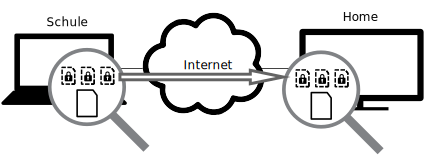
\includegraphics[]{images/sblit_p2p}
  \caption{Übertragung der Datei zwischen zwei erreichbaren Hosts}.
\end{figure}

\subsubsection{Synchronisieren zwischen zwei nicht erreichbaren \glspl{syncpartner}}
Für \glspl{syncpartner}, die nicht erreichbar sind, wird die Datei in der dezentralen
\gls{filecloud} zwischengespeichert. Die Datei wird kopiert und in Blöcke
aufgeteilt. Diese Blöcke werden verschlüsselt und verteilt auf den
\glspl{partnerdevice} gespeichert.

Da die Erreichbarkeit der gesamten Datei auf den Partnergeräten zu gewährleisten
ist, wird die Datei mehrmals
in die dezentrale \gls{filecloud} gespeichert, sodass nur ein Bruchteil der
Partnergeräte erreichbar sein muss, um auf die vollständige Datei zugreifen zu
können.

\begin{figure}[h]
	\centering
  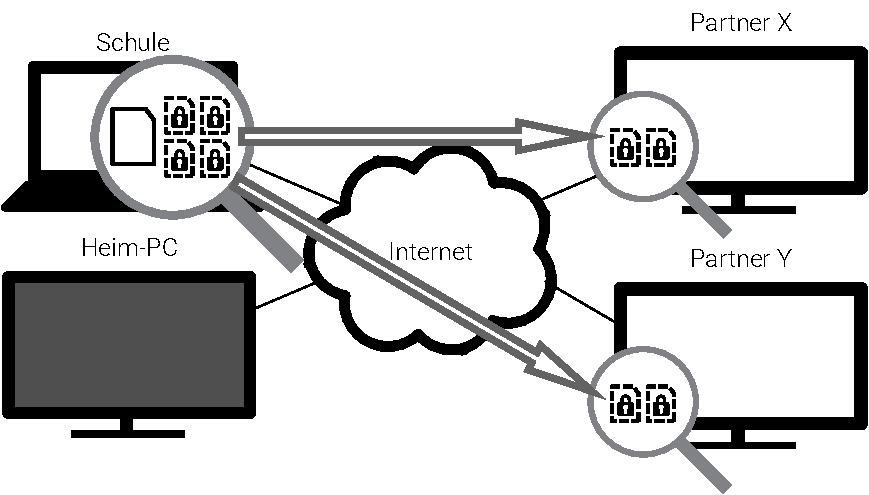
\includegraphics[]{images/sblit_upload}
  \caption{Hochladen der Datei in die dezentrale \gls{filecloud}}.
\end{figure}

Sobald der \gls{syncpartner}, hier der Heim-PC wieder hochgefahren ist, fordert er die
verschlüsselten Dateiblöcke von den \glspl{partnerdevice} an. Die Blöcke werden über
direkte verschlüsselte Verbindungen gesendet, entschlüsselt und zu der
vollständigen neuen Datei zusammengesetzt.

%Die Datei wurde somit über die aus den \glspl{partnerdevice} bestehende dezentrale
%\gls{filecloud} synchronisiert.

\begin{figure}[h]
	\centering
  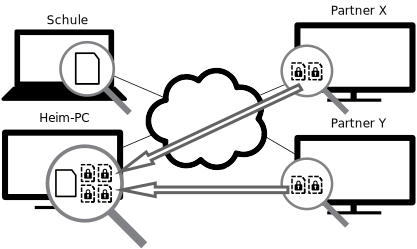
\includegraphics[]{images/sblit_download}
  \caption{Herunterladen der Datei aus der dezentralen \gls{filecloud} beziehungsweise
	den \glspl{partnerdevice}}.
\end{figure}
